\documentclass[Protokollheft.tex]{subfiles}
\begin{document}
	\chapter{Einführung in Numerische Methoden}
	%--------------- Start Vorbereitungsaufgaben ---------------
	
	\section{Vorbereitungsaufgaben}
	{\subsection{Differenzenverfahren}}
	
	% --> Aufgabe
	\begin{framed}
		\noindent \textbf{1.} Zeigen Sie, dass der zentrale Differenzenquotient (1.5) aus der Subtraktion zweier Taylor-Entwicklungen zu den Punkten $x_{i+1}$ und $x_{i-1}$ folgt. Vergessen Sie dabei nicht, die Fehlerterme zu berücksichtigen und kommentieren Sie die Ordnung des Fehlers im Vergleich zu vorwärts- und rückwärts-Differenzenquotient.\label{exer:diffquot}
	\end{framed}
	\noindent
	Der zentrale Differenzenquotient 
	\begin{equation}
	\label{eq:zentDif}
	f^{(1)}(x_i) = \frac{f(x_{i+1})-f(x_{i-1})}{\Delta x_{i-1}+\Delta x_i} + \mathcal{O}(\Delta x^{1\cdots2})
	\end{equation}
	
	setzt sich zusammen aus dem Vorwärts-Differenzenquotienten
	\begin{equation}
	\label{eq:vorDif}
	f^{(1)}(x_i) = \frac{f(x_{i+1})-f(x_{i})}{\Delta x_{i}} + \mathcal{O}(\Delta x)
	\end{equation}
	und dem Rückwärts-Differenzenquotienten
	\begin{equation}
	\label{eq:rueckDif}
	f^{(1)}(x_i) = \frac{f(x_{i})-f(x_{i-1})}{\Delta x_{i-1}} + \mathcal{O}(\Delta x)
	\end{equation}
	
	Im folgenden wird die Herleitung des Zentralen Differenzenquotienten bei homogenen Abständen $\Delta x$ dargestellt.\\
	Durch Subtraktion der Taylor Entwicklung zweiter Ordnung zu \ref{eq:rueckDif} von der Entwicklung zu \ref{eq:vorDif} ergibt sich 
	\begin{align}
		\label{eq:taylor}
		f(x_{i+1})-f(x_{i-1})& = &f(x_i)+\Delta x_i \cdot f'(x_i) + \mathcal{O} (\Delta x_i) 
		- (f(x_i) - \Delta x_{i-1}\cdot f'(x_i) + \mathcal{O} (\Delta x_{i-1})) \nonumber \\	
		& = & (\Delta x_i + \Delta x_{i-1}) f'(x_i) + \mathcal{O} (\Delta x_i \cdot \Delta x_{i-1})
	\end{align}
	Hieraus ergibt sich durch Umstellen nach $f'(x_i)$ der Zentrale Differenzenquotient \ref{eq:zentDif}. \\
	Der Fehler liegt zwischen $\mathcal{O}(\Delta x)$ und $\mathcal{O} (\Delta x^2)$ Abhängig vom Verhältnis der Abstände. Für äquidistante Abstände ist der Fehler $\mathcal{O} (\Delta x^2)$.
	
	
	% --> Aufgabe
	\begin{framed}
		\noindent \textbf{2.} Berechnen Sie ausgehend von einem Startpunkt \(f(\tilde{x}_i)\) auf einem dualen Gitter mit Hilfe von Taylorentwicklungen analog zur Differenzenvorschrift (1.6) im Fall äquidistanter Gitter eine zentrale Differenzenvorschrift vierter Ordnung zur Berechnung der ersten Ableitung. Verwenden Sie hierfür \(f(x_i), f(x_{i+1}), f(x_{i+2})\) sowie \(f(x_{i-1})\).\label{exer:diffquotOrd4}
	\end{framed}
	\noindent
	Um eine Differentiationsvorschrift vierter Ordnung für einen Startpunkt $\tilde{x_i}$ im dualen Gitter zu bestimmen wird ein lineares Gleichungssystem 
	\begin{align}
		\label{eq:dgl}
		f'(\tilde{x_i}) &= \frac{a(f(\tilde{x}_{i-\frac{h}{2}})-f(\tilde{x}_{i+\frac{h}{2}})+c(f(\tilde{x}_{i-\frac{3}{2}h})-f(\tilde{x}_{i+\frac{3}{2}h}))}{4h} \nonumber\\
		f({x_i}) & = f(\tilde{x_i}) - \frac{h}{2}f'(\tilde{x_i})+\frac{h^2}{8}f''(\tilde{x_i})-\frac{h^3}{48}f'''(\tilde{x_i}) + \mathcal{O}(h^4) \nonumber\\
		f({x_{i+1}}) & = f(\tilde{x_i}) + \frac{h}{2}f'(\tilde{x_i})+\frac{h^2}{8}f''(\tilde{x_i})+\frac{	h^3}{48}f'''(\tilde{x_i}) + \mathcal{O}(h^4)\\
		f({x_{i+2}}) & = f(\tilde{x_i}) + \frac{3h}{2}f'(\tilde{x_i})+\frac{9h^2}{8}f''(\tilde{x_i})+\frac{27h^3}{48}f'''(\tilde{x_i}) + \mathcal{O}(h^4) \nonumber\\
		f({x_{i-1}}) & = f(\tilde{x_i}) - \frac{3h}{2}f'(\tilde{x_i})+\frac{9h^2}{8}f''(\tilde{x_i})-\frac{27h^3}{48}f'''(\tilde{x_i}) + \mathcal{O}(h^4) \nonumber
	\end{align}
	mit $\Delta x = h$ aufgestellt. \\
	Hieraus folgt somit
	\begin{equation}
	\label{eq:LGS}
	f(x_{i+1} - f(x_i) = hf'(\tilde{x_i}) + \frac{1}{24}h^3 f'''(\tilde{x_i})+\mathcal{O}(h^4) 
	\end{equation}
	und
	\begin{equation}
	\label{eq:LGS2}
	f(x{i+2}) - f(x_{i-1})=3hf'(\tilde{x_i}) + \frac{27}{24}h^3f'''(\tilde{x_i}) + \mathcal{O}(h^4)
	\end{equation}
	
	Damit nun die 3.Ableitungen wegfallen wird ein Koeffizientenvergleich von $a$ und $c$ durchgeführt.
	Mit 
	\begin{align*}
		a[f(x_{i+1})-f(x_i)] =& a[hf'(\tilde{x_i}) + \frac{1}{24}h^3 f'''(\tilde{x_i})]+\mathcal{O}(h^4) \\
		c[f(x_{i+2})-f(x_{i-1})] =& c[3hf'(\tilde{x_i}) + \frac{27}{24}h^3f'''(\tilde{x_i}) ]+ \mathcal{O}(h^4)
	\end{align*}
	ergibt sich somit für $a = -27c$ 
	\begin{equation*}
		-27[f(x_{i+1})-f(x_i)]+[f(x_{i+2})-f(x_{i-1})] = -24 hf'(\tilde{x_i})
	\end{equation*}
	Woraus sich die Differenzenvorschrift vierter Ordnung zur Berechnung der ersten Ableitung zu 
	\begin{equation}
	\label{eq:DifVorOrd4}
	f'(\tilde{x_i}) = \frac{27[f(x_{i+1})-f(x_i)]-[f(x_{i+2})-f(x_{i-1})]}{24h}
	\end{equation}
	
	% --> Aufgabe
	\begin{framed}
		\noindent \textbf{3.} Bestimmen Sie aus der Differenzenvorschrift (1.10) die Matrix $\tilde{\textbf{C}}\textbf{C}$ für einen 1D-Resonator mit $5$~Stützstellen für den Fall elektrischer bzw. magnetischer Randbedingungen an beiden Rändern (siehe Abb.~1.3,~Gl.~(1.15)~und~Gl.~(1.16)).\label{exer:matrixCC}
	\end{framed}
	\noindent
	Nach (1.10) aus dem Skript ist der Differenzenquotient vierter Ordnung gegeben durch
	\begin{equation}
	\label{eq:DQ40}
	f^{(2)}(x_i)=\frac{16(f(x_{i+1})+f(x_{i-1}))-(f(x_{i+2})+f(x_{i-2}))-30f(x_i)}{12\Delta x^2}+\mathcal{O}(\Delta x^2).
	\end{equation}
	Betrachtet man weiterhin die eindimensionale Wellengleichung
	\begin{equation*}
		\frac{d^2\underline{E}_y}{dx^2}=-k^2_x\underline{E}_y
	\end{equation*}
	kann man nun den Differenzenquotienten aus (\ref{eq:DQ40}) in diese Gleichung einsetzten. Dazu werden die Funktionswerte in einen Vektor $\mathbf{e}$ geschrieben. Die Koeffizienten der Funktionswerte aus (\ref{eq:DQ40}) werden in der Matrix $\mathbf{\widetilde{C}C}$ gesammelt, sodass sich folgende Diskretisierung des Problems ergibt:
	\begin{equation}
	\label{eq:cc}
	\frac{1}{12}\mathbf{\widetilde{C}Ce}=-\Delta x^2k^2_x\mathbf{e}
	\end{equation}
	mit
	\begin{eqnarray*}
		\mathbf{e}&=&\left(\begin{array}{c} \vdots\\ f(x_{i-1})\\ f(x_i) \\ f(x_{i+1})\\
			\vdots\\\end{array}\right)\\
		\noindent
		\mathbf{\widetilde{C}C}&=&\begin{pmatrix} -30 & 16 & -1 & 0 & 0 & 0 & \dots \\ 
			16 & -30 & 16 & -1 & 0 & 0 & \dots\\ 
			-1 & 16 & -30 & 16 & -1 & 0 & \dots\\ 
			0 & -1 & 16 & -30 & 16 & -1 & \ddots\\ 
			\vdots & \ddots & \ddots & \ddots & \ddots & \ddots & \ddots\\
			\vdots & \vdots & \ddots & -1 & 16 & -30 & 16\\
			\vdots & \vdots & \vdots & 0 & -1 & 16 & -30\\
		\end{pmatrix}
	\end{eqnarray*}
	Die Matrix $\mathbf{\widetilde{C}C}$ beinhaltet aber noch keine Randbedingungen. Wir können zwei unterschiedliche Arten von Randbedingungen ansetzen. Einmal elektrische Randbedingungen und einmal magnetische Randbedingungen. Bei elektrischen Randbedingungen gilt eine ungerade Symmetrie, das heißt, dass wenn sich $f(x_0)$ am Rand befindet $(f(x_{-1})=-f(x_{1}))$ gilt. Bei magnetischen Randbedingungen gilt im Gegensatz dazu eine gerade Symmetrie mit $(f(x_{-1})=f(x_{1}))$. Will man nun die Randbedingungen einpflegen, so muss man jeweils die ersten und letzten beiden Zeilen anpassen.\\
	Für elektrische Randbedingungen in den ersten beiden Zeilen gilt folgendes:
	\begin{eqnarray*}
		-\frac{1}{12}f(x_{-2})+\frac{16}{12}f(x_{-1})-\frac{30}{12}f(x_0)+\frac{16}{12}f(x_{1})-\frac{1}{12}f(x_{2})&=&-\Delta x^2k^2_xf(x_0)\\
		-\frac{30}{12}f(x_0)&\stackrel{ung. Symm.}{=}&-\Delta x^2k^2_xf(x_0)\\
		\\
		\\
		-\frac{1}{12}f(x_{-1})+\frac{16}{12}f(x_{0})-\frac{30}{12}f(x_1)+\frac{16}{12}f(x_{2})-\frac{1}{12}f(x_{3})&=&-\Delta x^2k^2_xf(x_1)\\
		\frac{16}{12}f(x_{0})-\frac{29}{12}f(x_1)+\frac{16}{12}f(x_{2})-\frac{1}{12}f(x_{3})&\stackrel{ung. Symm.}{=}&-\Delta x^2k^2_xf(x_1)\\
	\end{eqnarray*}
	Bei magnetischen Randbedingungen gilt dagegen:
	\begin{eqnarray*}
		-\frac{1}{12}f(x_{-2})+\frac{16}{12}f(x_{-1})-\frac{30}{12}f(x_0)+\frac{16}{12}f(x_{1})-\frac{1}{12}f(x_{2})&=&-\Delta x^2k^2_xf(x_0)\\
		-\frac{30}{12}f(x_0+\frac{32}{12}f(x_{1})-\frac{2}{12}f(x_{2}))&\stackrel{g. Symm.}{=}&-\Delta x^2k^2_xf(x_0)\\
		\\
		\\
		-\frac{1}{12}f(x_{-1})+\frac{16}{12}f(x_{0})-\frac{30}{12}f(x_1)+\frac{16}{12}f(x_{2})-\frac{1}{12}f(x_{3})&=&-\Delta x^2k^2_xf(x_1)\\
		\frac{16}{12}f(x_{0})-\frac{31}{12}f(x_1)+\frac{16}{12}f(x_{2})-\frac{1}{12}f(x_{3})&\stackrel{g. Symm.}{=}&-\Delta x^2k^2_xf(x_1)\\
	\end{eqnarray*}
	Das Ganze gilt analog für die letzten Beiden Zeilen der $\mathbf{\widetilde{C}C}$-Matrix, jedoch gespiegelt für den rechten Rand.
	Damit lassen sich die Matrizen für elektrische bzw. magnetische Randbedingungen aufstellen:
	\begin{eqnarray*}
		\mathbf{\widetilde{C}C}_{elek}&=&\begin{pmatrix} -30 & 0 & 0 & 0 & 0 & 0 & \dots \\ 
			16 & -29 & 16 & -1 & 0 & 0 & \dots\\ 
			-1 & 16 & -30 & 16 & -1 & 0 & \dots\\ 
			0 & -1 & 16 & -30 & 16 & -1 & \ddots\\ 
			\vdots & \ddots & \ddots & \ddots & \ddots & \ddots & \ddots\\
			\vdots & \vdots & \ddots & -1 & 16 & -29 & 16\\
			\vdots & \vdots & \vdots & 0 & 0 & 0 & -30\\
		\end{pmatrix}
		\\
		\\
		\\
		\\
		\mathbf{\widetilde{C}C}_{magn}&=&\begin{pmatrix} -30 & 32 & -2 & 0 & 0 & 0 & \dots \\ 
			16 & -31 & 16 & -1 & 0 & 0 & \dots\\ 
			-1 & 16 & -30 & 16 & -1 & 0 & \dots\\ 
			0 & -1 & 16 & -30 & 16 & -1 & \ddots\\ 
			\vdots & \ddots & \ddots & \ddots & \ddots & \ddots & \ddots\\
			\vdots & \vdots & \ddots & -1 & 16 & -31 & 16\\
			\vdots & \vdots & \vdots & 0 & -2 & 32 & -30\\
		\end{pmatrix}
	\end{eqnarray*}
	
	% --> Aufgabe
	\begin{framed}
		\noindent \textbf{4.} Betrachtet werden soll exemplarisch die Berechnung der diskreten Wellenzahlen bei vorgegebener Länge des Rechengebietes nach Gl.~(1.14).
		Geben Sie den Abbruchfehler in Abhängigkeit von der Anzahl der verwendeten Stützstellen $n$ bzw. der Diskretisierungsschrittweite $\Delta x$ an,
		wenn der Differenzenquotient nach Gl.~(1.9) bzw. Gl.~(1.10) verwendet wird.
		Wie müssen Sie ein entsprechendes Diagramm (Abbruchfehler vs. Anzahl der Stützstellen) skalieren, um einen geradlinigen Verlauf zu erhalten?\label{exer:failureTerm}
	\end{framed}
	\noindent
	Ergänzt man (\ref{eq:cc}) mit dem Fehler $\mathcal{O}(\Delta x^2)$ so erhält man
	\begin{equation}
	\frac{1}{12\Delta x^2}\mathbf{\widetilde{C}Ce}+k^2_x\mathbf{e}+\mathcal{O}(\Delta x^4)=0
	\end{equation}
	Der Fehler dieser Gleichung liegt also in der Ordnung $\mathcal{O}(\Delta x^4)$. Mit $\Delta x=\frac{L}{n-1}$, wobei L die Länge des Rechengebietes und n die Anzahl der Stützstellen ist. Damit kann man die Ordnung ganz einfach in Abhängigkeit der Stückstellenanzahl schreiben. $\mathcal{O}(\frac{1}{(n-1)^4})$ ist hierbei nicht von L anhängig, da dies nur eine Konstante darstellt.\\
	Diese Rechnung beschreibt das Vorgehen mit dem in (\ref{eq:DQ40}) gezeigt Differenzenquotient vierter Ordnung. Das Ganze funktioniert analog mit dem Differenzenquotieten zweiter Ordnung
	\begin{equation*}
		f^{(2)}(x_i)=\frac{f(x_{i+1})+f(x_{i-1})-2f(x_i)}{\Delta x^2}+\mathcal{O}(\Delta x^2)
	\end{equation*}
	wobei sich hier dann die Ordnung $\mathcal{O}(\frac{1}{(n-1)^2})$ ergibt.\\
	Will man einen gradlinigen Verlauf des Fehlers erhalten, so sollte man ihn doppel-logarithmisch plotten, weil dadurch der Exponent des Terms $(n-1)$ nur als einfacher Faktor berücksichtigt wird.
	
	% --> Aufgabe
	\begin{framed}
		\noindent \textbf{5.} Stellen Sie eine Formel auf, mit der die analytischen Wellenzahlen $k_{x,\,\text{ana}}$ für die eindimensionale Wellengleichung und
		einem Resonator der Länge~\(L\) einmal mit rein elektrischer Berandung und einmal mit unterschiedlichen Randbedingungen
		(eine Seite elektrisch -- eine Seite magnetisch) berechnet werden kann. Bestimmen Sie dabei auch die jeweils kleinste Wellenzahl.
		Geben Sie bei einer numerischen Berechnung eine Formel für den relativen Wellenzahlfehler $\Delta k_{x}$ an.\label{exer:kxAnalytic}
	\end{framed}
	\noindent
	Zur Bestimmung der Wellenzahlen $k_{x,\,\text{ana}}$ betrachten wir wieder 
	\begin{equation*}
		\frac{\text{d}\underline{E}_y}{\text{d}x^2}+k^2_x\underline{E}_y=0.
	\end{equation*}
	Zur Lösung dieser gewöhnlichen Differentialgleichung 2. Ordnung wählt man den Ansatz
	\begin{equation}
	\label{eq:ansatz}
	\underline{E}_y=c_1 \text{cos}(k_xx)+c_2 \text{sin}(k_xx)
	\end{equation}
	Im Fall beidseitiger elektrischer Randbedingungen ergeben sich folgende Randbedingungen für $\underline{E}_y$:
	\begin{eqnarray*}
		(\text{I}) \ \ \ \underline{E}_y(0)&=&0\\
		(\text{II}) \ \ \ \underline{E}_y(L)&=&0\\
	\end{eqnarray*}
	Mit (I) und (\ref{eq:ansatz}) folgt direkt $c_1=0$. Mit (II) und (\ref{eq:ansatz}) folgt $c_2$sin$(k_xL)=0$. Damit dies erfüllt wird muss $k_x=\frac{n\pi}{L}$ mit $n \in\mathbb{Z}$ gelten. Mit $c_2=0$ wird die triviale Nulllösung erreicht, aber man will alle möglichen Lösungen finden. Die kleinste Wellenzahl ist damit $k_x=\frac{\pi}{L}$.\\
	\\
	Im Fall, das eine Seite eine elektrische und eine Seite eine magnetische Randbedingung besitzt, sehen die Randbedingungen folgendermaßen aus:
	\begin{eqnarray*}
		(\text{I}) \ \ \ \underline{E}_y(0)&=&0\\
		(\text{II}) \ \ \ \underline{H}_x(L)&=&0\\
	\end{eqnarray*}
	Für (II) kann man das Faraday'sche Gesetz im Frequenzbereich $\text{rot}\underline{E}_y=-j\omega\mu \underline{H}_x$ verwenden. Da die Rotation im eindimensionalen nur eine einfach Ableitung beschreibt, kann man $\frac{\text{d}\underline{E}_y}{\text{d}x}\propto\underline{H}_x$ schreiben. Damit folgt aus (II)
	\begin{equation*}
		(\text{III}) \ \ \ \frac{\text{d}\underline{E}_y(L)}{\text{d}x}=0\\.
	\end{equation*}
	Verwendet man nun wieder (\ref{eq:ansatz}) und (I) ergibt sich $c_1=0$. Mit (III) und (\ref{eq:ansatz}) ergibt sich $c_2k_x\text{cos}(k_xL)=0$ mit $n \in\mathbb{Z}$. Damit dies erfüllt wird muss $k_x=\frac{\pi}{L}(\frac{n}{2}+1)$ gelten. $c_2=0$ wäre die einfache triviale Lösung. Die kleinste Wellenzahl ist damit $k_X=\frac{\pi}{L}$.
	
	
	
	
	% --> Aufgabe
	\begin{framed}
		\noindent \textbf{6.} Wie kann man die Orthogonalität zweier Eigenvektoren testen und was sagen orthogonale Eigenvektoren über die Lösungen eines Eigenwertproblems (Moden) aus?\label{exer:orthogonalEV}
	\end{framed}
	\noindent
	Die Eigenvektoren können durch Bildung des Skalarproduktes und Überprüfung $\vec{A} \cdot \vec{B} = 0$ auf Orthogonalität getestet werden. \\
	Orthogonalität der Eigenvektoren bedeutet, dass alle Moden senkrecht zueinander stehen.
	
	\noindent{\subsection{Dreidimensionale Darstellung}}
	
	\noindent Gegeben sei in Abbildung \ref{fig:zylGitter} die Diskretisierung eines Kreiszylinders der Höhe $h$ und des Radius $r$ mit $n_\mathrm{D}$ Deckflächendreiecken der Grundlänge $2a_\text{D}$ und Höhe $h_\text{D}$.\\
	\begin{figure}[h]
		\centering
		\begin{subfigure}{0.49\textwidth}
			\centering
			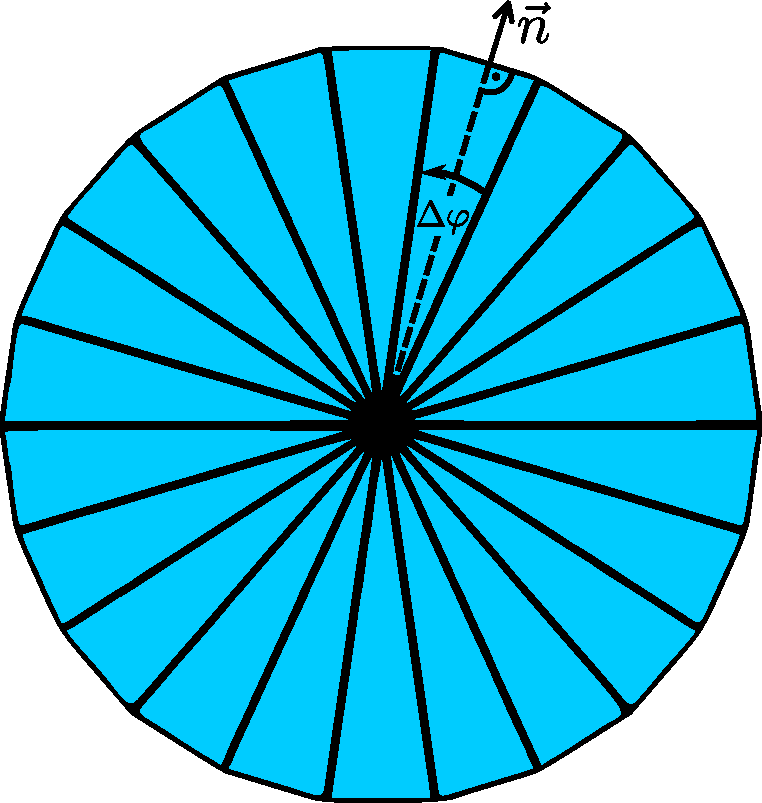
\includegraphics[height=4.5cm]{v1_zylinder1.pdf}
		\end{subfigure}
		\begin{subfigure}{0.49\textwidth}
			\centering
			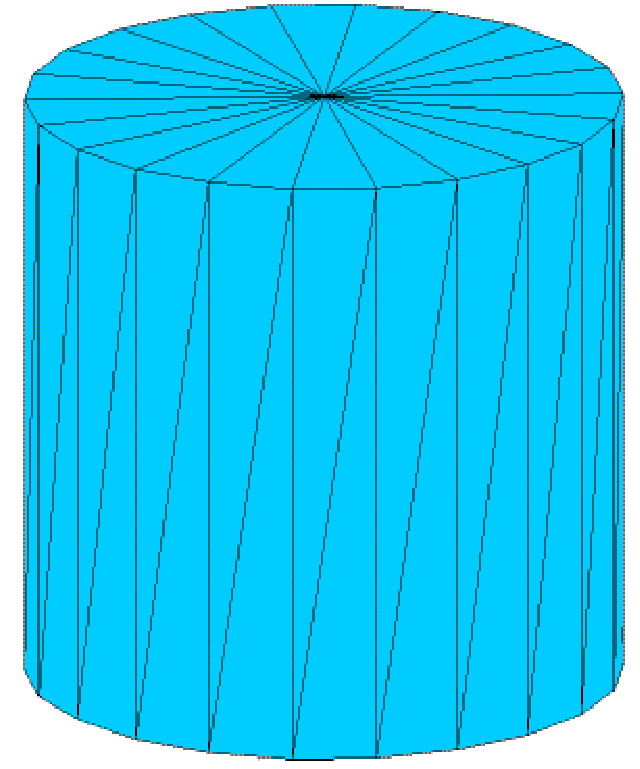
\includegraphics[height=4.5cm]{v1_zylinder2.pdf}
		\end{subfigure}
		\caption{Diskretisierung einer Kreiszylinderoberfläche. Dargestellt sind die Dreiecksgitter der Diskretisierung der Deckelfläche (links) und des diskretisierten Zylinders in Perspektivansicht (rechts).}\label{fig:zylGitter}
	\end{figure}
	
	
	
	% --> Aufgabe
	\begin{framed}
		\noindent \textbf{7.} Überlegen Sie sich einen Pseudocode mit For-Schleifen, mit welchem Sie die Koordinaten aller Dreiecke der Oberflächendiskretisierung (siehe Abb.~\ref{fig:zylGitter}) bestimmen können. Die Anzahl der Dreiecke~$n_\text{D}$ soll dabei beliebig sein. Beachten Sie, dass zur Oberfläche Deck-, Mantel- und Bodenfläche gehören. Außerdem besitzen die Dreiecke auf der Mantelfläche \glqq unterschiedliche Orientierungen\grqq.\label{exer:pseudocodeCylinder}
	\end{framed}
	\noindent
	Um die Koordinaten aller Dreiecke in Abhängigkeit von $n_\text{D}$ zu bestimmen, wird zunächst der Deckel betrachtet. Ein Punkt am Rand des Deckels hat immer die Koordinaten 
$	\begin{pmatrix}
		r\text{cos}(i\Delta\varphi)\\
		r\text{sin}(i\Delta\varphi)\\
		h
	\end{pmatrix}$.
	Dabei beschreibt $\Delta\varphi$ den Winkel wischen 2 Dreiecksseiten. Dieser ergibt sich aus $\Delta\varphi=\frac{2\pi}{n_D}$. Das $i$ beschreibt den Laufindex für die for-Schleife. Hat das Dreieck als Koordinaten von 2 Punkten 
	$\begin{pmatrix}
		0\\
		0\\
		h
	\end{pmatrix}$,
	$\begin{pmatrix}
		r\text{cos}(i\Delta\varphi)\\
		r\text{sin}(i\Delta\varphi)\\
		h
	\end{pmatrix}$ gegeben, so ist der dritte Punkt gegeben durch
$	\begin{pmatrix}
		r\text{cos}(i\Delta\varphi+\Delta\varphi)\\
		r\text{sin}(i\Delta\varphi+\Delta\varphi)\\
		h
	\end{pmatrix}$.
	Diese Punkte werden nun mit einer for-Schleife abgetastet und gespeichert. Das gleiche geschieht auch mit den Dreiecken am Boden des Zylinders, nur, dass die z-Koordinate hier immer 0 ist.\\
	Für den Mantel gilt es jetzt nur die Schon berechneten Punkte wiederzuverwerten. Dreiecke bei denen 2 Punkte am Boden und einer am Deckel ist, müssen einen Punkt von Boden, den darauf folgenden Punkt sowie den Punkt, der in der Höhe $h$ im Vergleich zum ersten Punkt liegt abspeichern. Für die Dreiecke, die andersherum orientiert sind gilt das gleiche, nur sind hier Deckel und Boden vertauscht. 
	
	
	% --> Aufgabe
	\begin{framed}
		\noindent \textbf{8.} In der Theorie wurde erwähnt, dass eine feinere Diskretisierung die Genauigkeit der Darstellung steigert\footnote{Es gibt jedoch Fälle, bei denen eine Verdichtung des Oberflächengitters nicht gegen die exakte Lösung konvergiert.}, aber dass auch der Rechenaufwand und der geforderte Speicher zunehmen.
		Berechnen Sie den Speicherplatz, der zur Speicherung des oben abgebildeten, diskretisierten Zylinders im STL-Format notwendig ist, als Funktion der Anzahl der Dreiecke $n_\mathrm{D}$ (Normalenvektoren müssen auch berücksichtigt werden). Beachten Sie hierbei lediglich die notwendige Anzahl der \lstinline{double}-Zahlen, wobei eine \lstinline{double}-Zahl \SI{8}{Byte} benötigt.\label{exer:requiredStorage}
	\end{framed}
	\noindent
	Im STL Format ist jedes Dreieck durch 3 Punkte und einen Normalenvektor beschrieben. Jeder Punkt und jeder Normalenvektor hat 3 Koordinaten. Dazu besteht jeder Zylinder aus $4 \cdot n_\text{D}$ Dreiecken.\\
	Damit kann man den benötigte Speicherplatz zu 
	\begin{eqnarray*}
		\text{Speicher}(n_\mathrm{D})&=&4n_\mathrm{D}(3\text{ Punkte + Normalenvektor})\cdot 3 \text{ Koordinaten.}\cdot 8\text{ Bytes}\\
		&=&384n_\mathrm{D} \text{ Bytes}
	\end{eqnarray*}
	bestimmen. 
	% --> Aufgabe
	\begin{framed}
		\noindent \textbf{9.} Gegeben ist folgender Zusammenhang für die Fläche eines Deckflächendreieckes:
		\begin{align}
			A_\text{D} &= 2 \left[\frac12 a_\text{D} h_\text{D}\right] = 2 \left[ \frac12 \cdot r \cos\left(\frac{\Delta \varphi}{2}\right)\cdot r \sin\left(\frac{\Delta \varphi}{2}\right)  \right] = \frac12 r^2 \sin(\Delta\varphi)
		\end{align}
		Überlegen sie sich geometrisch, wie diese Formel zustande kommt und dokumentieren Sie die einzelnen Schritte. Leiten Sie anschließend eine Formel zur Berechnung des Volumens und der Fläche des gezeigten Zylinders in Abhängigkeit von der Anzahl der Deckflächendreiecke $n_\mathrm{D}$ her.\\
		Bestimmen Sie den relativen Oberflächenfehler $\Delta A$ bzw. Volumenfehler $\Delta V$ dieser Diskretisierung.
		Bei welchen Körpern wäre eine solche Oberflächendiskretisierung mit Dreiecken exakt?\label{exer:deltaAdeltaV}
	\end{framed}
	\noindent
	Ein Dreieck der Deckfläche ist ein gleichschenkliges Dreieck. Um die Fläche des gleichschenkliges Dreieckes zu bestimmen, soll man es mithilfe der Höhe  $h_\text{D}$ in zwei rechtwinklige Dreiecke teilen. Die Fläche der rechtwinkliger Dreieck errechnet sich als Multiplikation zweier Katheten geteilt durch $2$. Damit bekommt man die Formel: 
	$$ A_\text{D} = 2 \left[\frac12 a_\text{D} h_\text{D}\right]$$
	Mit der Pythagoras Formel rechnet ergibt sich aus $h_\text{D}$ und $a_\text{D}$ :
	\begin{eqnarray*}
		a_\text{D}&=&r \sin\left(\frac{\Delta \varphi}{2}\right)\\
		\\
		h_\text{D}&=&r \cos\left(\frac{\Delta \varphi}{2}\right)
	\end{eqnarray*}
	Jetzt setzt man alles zusammen:
	$$A_\text{D} = 2 \left[ \frac12 \cdot r \cos\left(\frac{\Delta \varphi}{2}\right)\cdot r \sin\left(\frac{\Delta \varphi}{2}\right)  \right]$$
	Mithilfe der Sinusdoppelwinkelformel
	$$  \sin(\Delta\varphi)=2 \cos\left(\frac{\Delta \varphi}{2}\right) \sin\left(\frac{\Delta \varphi}{2}\right)  $$
	kann man der Formel noch vereinfachen auf:
	$$A_\text{D} =  \frac12 r^2 \sin(\Delta\varphi)$$
	
	Wenn man den relativen Oberflächen- und Volumenfehler bestimmen wollte, soll man die Oberfläche und das Volumen des wahres und des diskretisiertes Zylinders ausrechnen.
	\begin{eqnarray*}
		A_\text{disc}&=&2n_\text{D}r\left[ \frac12 \cdot r \sin\left(\frac{2 \pi}{n_\text{D}}\right)+ \sin\left(\frac{\pi}{n_\text{D}}\right)h  \right]\\
		\\
		V_\text{disc}&=&\frac12 n_\text{D} r^2 \sin\left(\frac{ 2\pi}{n_\text{D}}\right)h\\
		\\
		A&=&2 r \pi (r+h)\\
		\\
		V&=&r^2\pi h
	\end{eqnarray*}
	Die Formel für den absolute Fehler lautet\\
	$$\Delta X = X- X_\text{disc}$$.
	Damit bekommt man
	\begin{eqnarray*}
		\Delta A&=&2 r \pi (r+h) -2n_\text{D}r\left[ \frac12 \cdot r \sin\left(\frac{2 \pi}{n_\text{D}}\right)+ \sin\left(\frac{\pi}{n_\text{D}}\right)h  \right]\\
		\\
		\Delta V&=&r^2\pi h -\frac12 n_\text{D} r^2 \sin\left(\frac{ 2\pi}{n_\text{D}}\right)h\\
	\end{eqnarray*}.
	Den relative Fehler bekommt man mit der Formel:
	$$\varepsilon_{x}=\frac{\Delta X}{X}$$
	Damit bekommt man
	\begin{eqnarray*}
		\varepsilon_{A}&=&\frac{ \pi (r+h) -n_\text{D}\left[ \frac12 \cdot r \sin\left(\frac{2 \pi}{n_\text{D}}\right)+ \sin\left(\frac{\pi}{n_\text{D}}\right)h  \right]}{\pi (r+h)}\\
		\\
		\varepsilon_{V}&=&\frac{\pi  -\frac12 n_\text{D}  \sin\left(\frac{ 2\pi}{n_\text{D}}\right)}{\pi}
	\end{eqnarray*}
	% --> Aufgabe
	\begin{framed}
		\noindent \textbf{10.} Bei einigen Anwendungen ist es wichtig, dass die diskretisierte Fläche möglichst glatt bleibt. Ein
		wichtiges Beispiel hierbei ist die Streuung hochfrequenter elektromagnetischer Felder, wobei
		Kanten und Ecken das gestreute Feld verändern können. Angenommen bei der oberen
		Diskretisierung des Zylinders ist der Winkel zwischen den Normalenvektoren benachbarter Dreiecke der Deckflächen $\Delta \varphi \leq 5^{\circ}$ gefordert.
		Berechnen Sie die minimale Anzahl an Dreiecken zur Erfüllung dieser Forderung.\label{exer:smoothArea}
	\end{framed}
	\noindent
	Dieser Forderung rechnet man mit der schon bekannten Formel
	\ref{exer:pseudocodeCylinder}:
	$$\Delta \varphi = \frac{360^\circ}{n_\text{D}}$$ aus. 
	Realisierung der Forderung:
	\begin{eqnarray*}
		5^{\circ} &\geq& \frac{360^\circ}{n_\text{D}}\\
		\\
		n_\text{D} &\geq& 72
	\end{eqnarray*}
	
	Es werden minimal 72 Dreiecke benötigt.
	
	\section{Aufgaben während der Praktikumssitzung}
	{\subsection{Differenzenverfahren}}
	
	% --> Aufgabe
	\begin{framed}
		\noindent \textbf{1.} Implementieren Sie eine Methode
		\begin{align}
			\lstinline{[cc] = createCC(n, ord, bc)}\; \label{meth:createCC}
		\end{align}     
		welche die $\tilde{\textbf{C}}\textbf{C}$-Matrix mit der Stützstellenanzahl \lstinline{n}, der Ordnung des Differenzenverfahrens
		\lstinline{ord}\\ (\lstinline{2} = zweite und \lstinline{4} = vierte Ordnung) und der für beide Ränder identischen Art der Randbedingung \lstinline{bc} (\lstinline{0=}fehlende, \lstinline{1=}elektrische und  \lstinline{2=}magnetische) erstellt.
		Rückgabewert ist die $\tilde{\textbf{C}}\textbf{C}$-Matrix \lstinline{cc}. Nutzen Sie hierfür das vorgefertigte Template \lstinline{createCC.m}.\label{exer:createCC}
	\end{framed}
	
	%\lstinputlisting {createCC.m}
	
	% --> Aufgabe
	\begin{framed}
		\noindent \textbf{2.} Ein einfacher Solver soll in
		\begin{align}
			\lstinline{[kx, modes] = solveCC(cc, dx)} \label{meth:solveCC}
		\end{align}
		implementiert werden, wobei die Schrittweite \lstinline{dx} als zusätzlicher Eingabeparameter übergeben wird.
		\lstinline{kx} ist hier ein Vektor mit den geordneten Wellenzahlen, angefangen mit der kleinsten Wellenzahl. In gleicher
		Reihenfolge sollen auch die Eigenvektoren in der Matrix \lstinline{modes} zurückgegeben werden.
		Das Eigenwertproblem lässt sich durch die \matlab-Funktion \lstinline{eig} lösen, das Sortieren kann mit \lstinline{sort} erfolgen.\label{exer:solveCC}
	\end{framed}
	
	%\lstinputlisting {solveCC.m}
	
	% --> Aufgabe
	\begin{framed}
		\noindent \textbf{3.} Verwenden Sie die Routine \lstinline{createCC} mit \lstinline{n=6},~\lstinline{ord=2} und \lstinline{bc=0} und anschließend \lstinline{solveCC}.
		Überprüfen Sie die Orthogonalität der Eigenvektoren. Wie viele Eigenmoden können bei dieser Parameterwahl bestimmt werden? Nutzen Sie hierfür die bereits gegebene Datei \lstinline{check_orth.m}.
		
		{\textbf{Hinweis:}} Wenn Sie die Eigenvektoren geschickt miteinander multiplizieren, erhalten Sie eine Matrix, in der jeder Eintrag einem Produkt zweier Eigenvektoren entspricht. Diese sich ergebene Matrix lässt sich dann bequem mit dem Befehl \verb\imagesc\ (siehe Abschnitt~1.1.3) darstellen.\label{exer:check_orth}
	\end{framed}
	
	%\lstinputlisting {check_orth.m}
	Mit der Routine \texttt{check\_orth} und den gegebenen Parametern konnten 6 Eigenmoden bestimmt werden. 
	
	% --> Aufgabe
	\begin{framed}
		\noindent \textbf{4.} Stellen Sie die zwei niedrigsten Moden in einem Skript \lstinline{plotModes} grafisch dar.
		Verwenden Sie \lstinline{n=100}, \lstinline{bc=1} und \lstinline{ord=4} sowie die Länge des eindimensionalen Gebietes L=\SI{5}{m}.\label{exer:plotModes}
	\end{framed}
	
	%\lstinputlisting {plotModes.m}
	\begin{figure}[h]
		\centering
		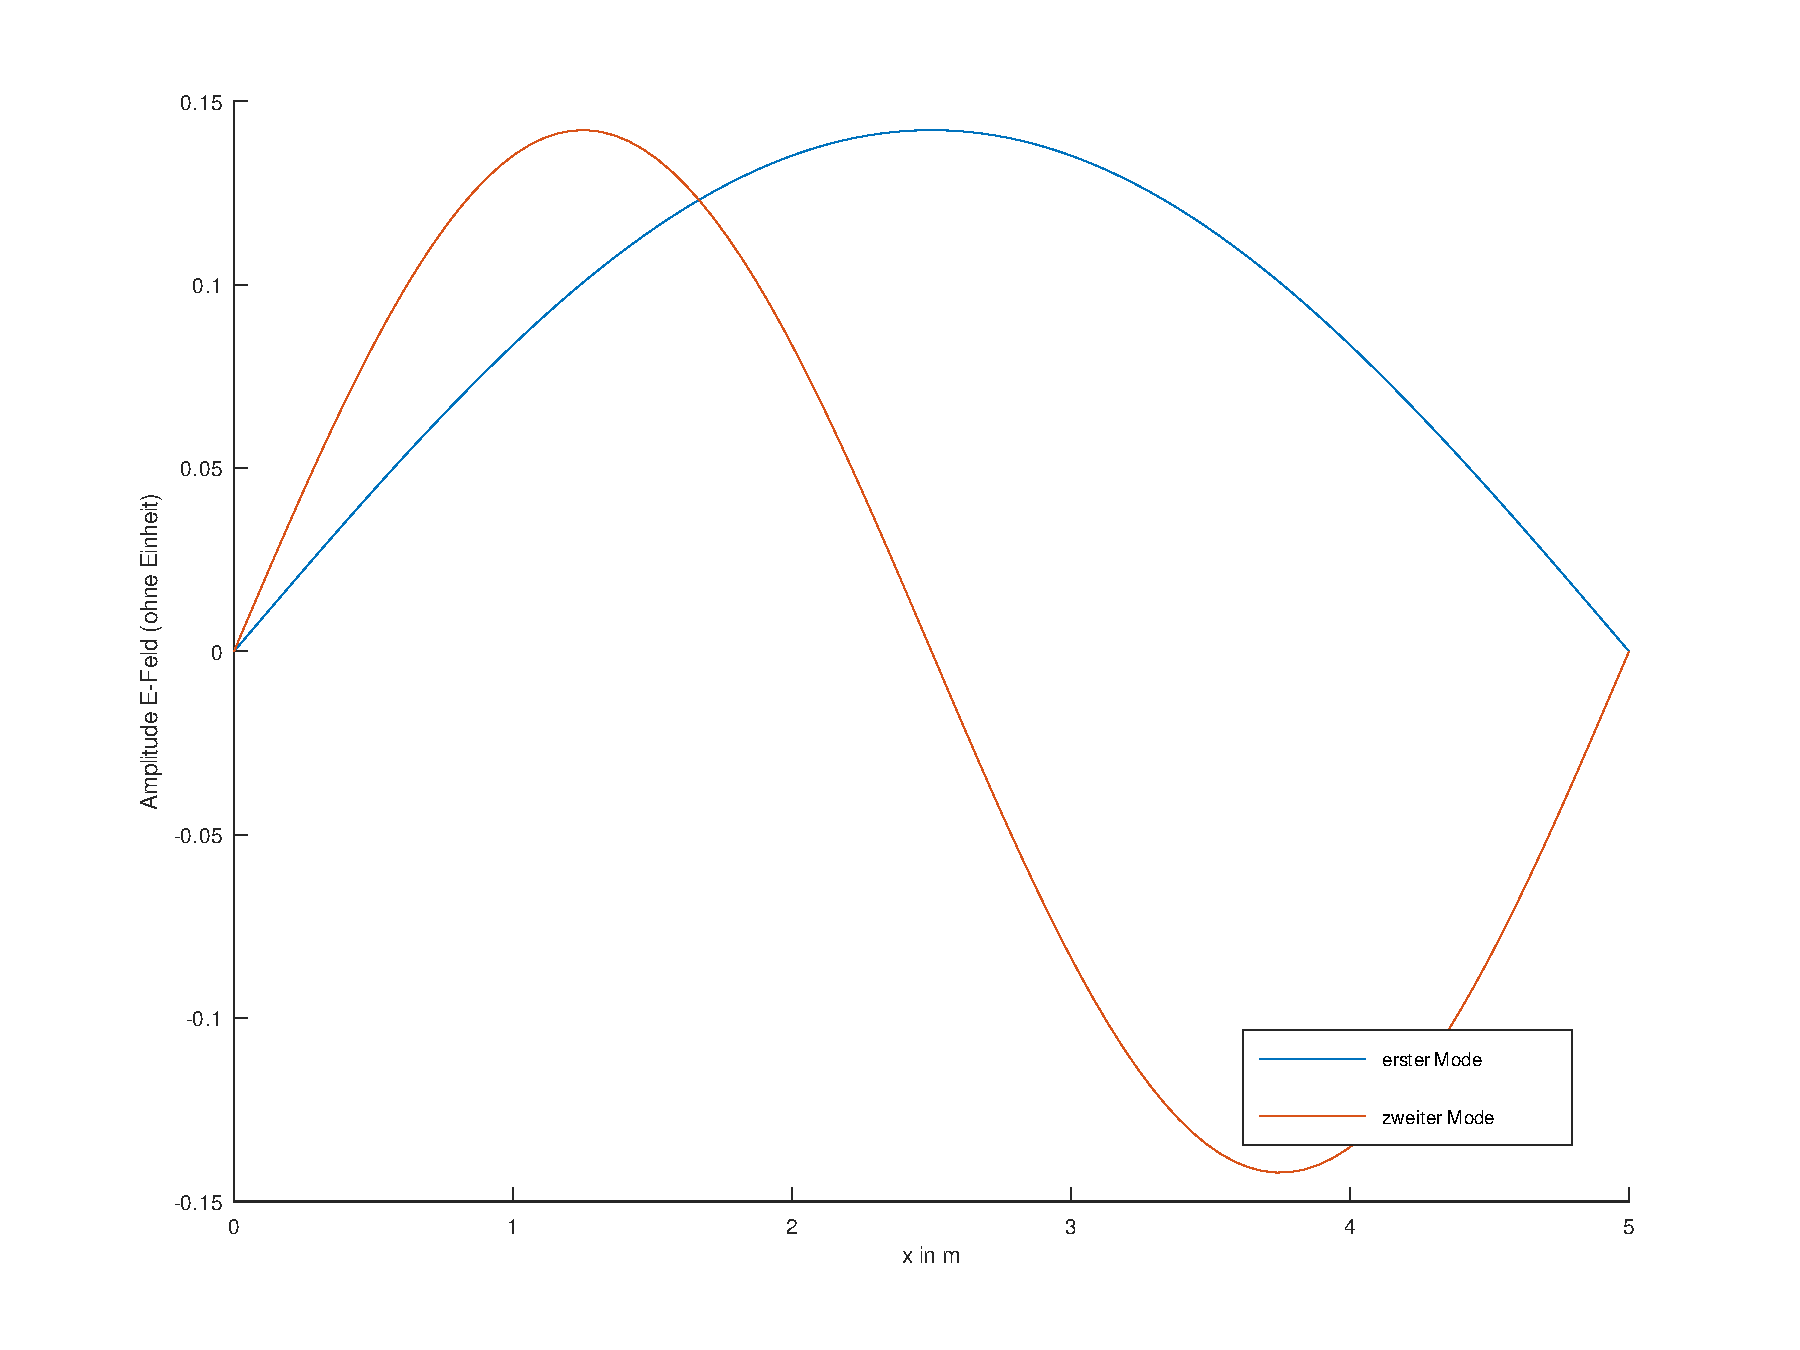
\includegraphics[trim = 20mm 15mm 20mm 15mm, clip, width=0.7\textwidth]{modes.pdf}
		\caption{Plot der zwei Moden mit der geringsten Frequenz.}
		
	\end{figure}
	
	% --> Aufgabe
	\begin{framed}
		\noindent \textbf{5.} Als nächstes sollen Sie das Konvergenzverhalten betrachten. Schreiben Sie ein Skript \lstinline{plotConv}, welches das Konvergenzverhalten in Abhängigkeit von der Stützstellenanzahl \lstinline{n}
		Ihrer verschiedenen Implementierungen in zwei Grafiken dokumentiert:
		\begin{enumerate}
			\item Lineare Darstellung der Wellenzahl des Grundmodes über der Stützstellenanzahl $n$ im Fall elektrischer Randbedingungen, sowohl analytisch als auch zweite und vierte Ordnung.
			\item Doppelt-logarithmische Darstellung des relativen Wellenzahlfehlers des Grundmodes  über die Gitterschrittweite bei elektrischen und fehlenden Randbedingungen für jeweils beide Ordnungen.
		\end{enumerate}
		Verwenden Sie die Grafiken um die Ordnung der verschiedenen Implementierungen graphisch zu bestimmen. Vergleichen Sie Ihr Ergebnis
		mit Aufgabe~\ref{exer:failureTerm} aus der Vorbereitung.  Wie verändert sich das Konvergenzverhalten, wenn keine Randbedingungen implementiert sind?\label{exer:plotConv}
	\end{framed}
	\noindent
	In Abbildung \ref{Abb:plotCov} wird eine Approximation der Wellenzahl an Abhängigkeit der Stützstellenanzahl des Gitters mit verschiedenen Verfahren dargestellt. In Abbildung \ref{Abb:plotCovloglog} wird der Wellenzahlfehler in Abhängigkeit der Gitterschrittweite gezeigt. Das Konvergenzverhalten wird durch die nicht gegebenen Randbedingungen schlechter. Dies ist auch logisch, da durch die vorgegebenen Werte an den Rändern nicht mehr so viele Möglichkeiten für Lösungen existieren. Dadurch konvergiert ein Verfahren mit Randbedingungen schneller als ohne. 
	\begin{figure}[h]
		\centering
		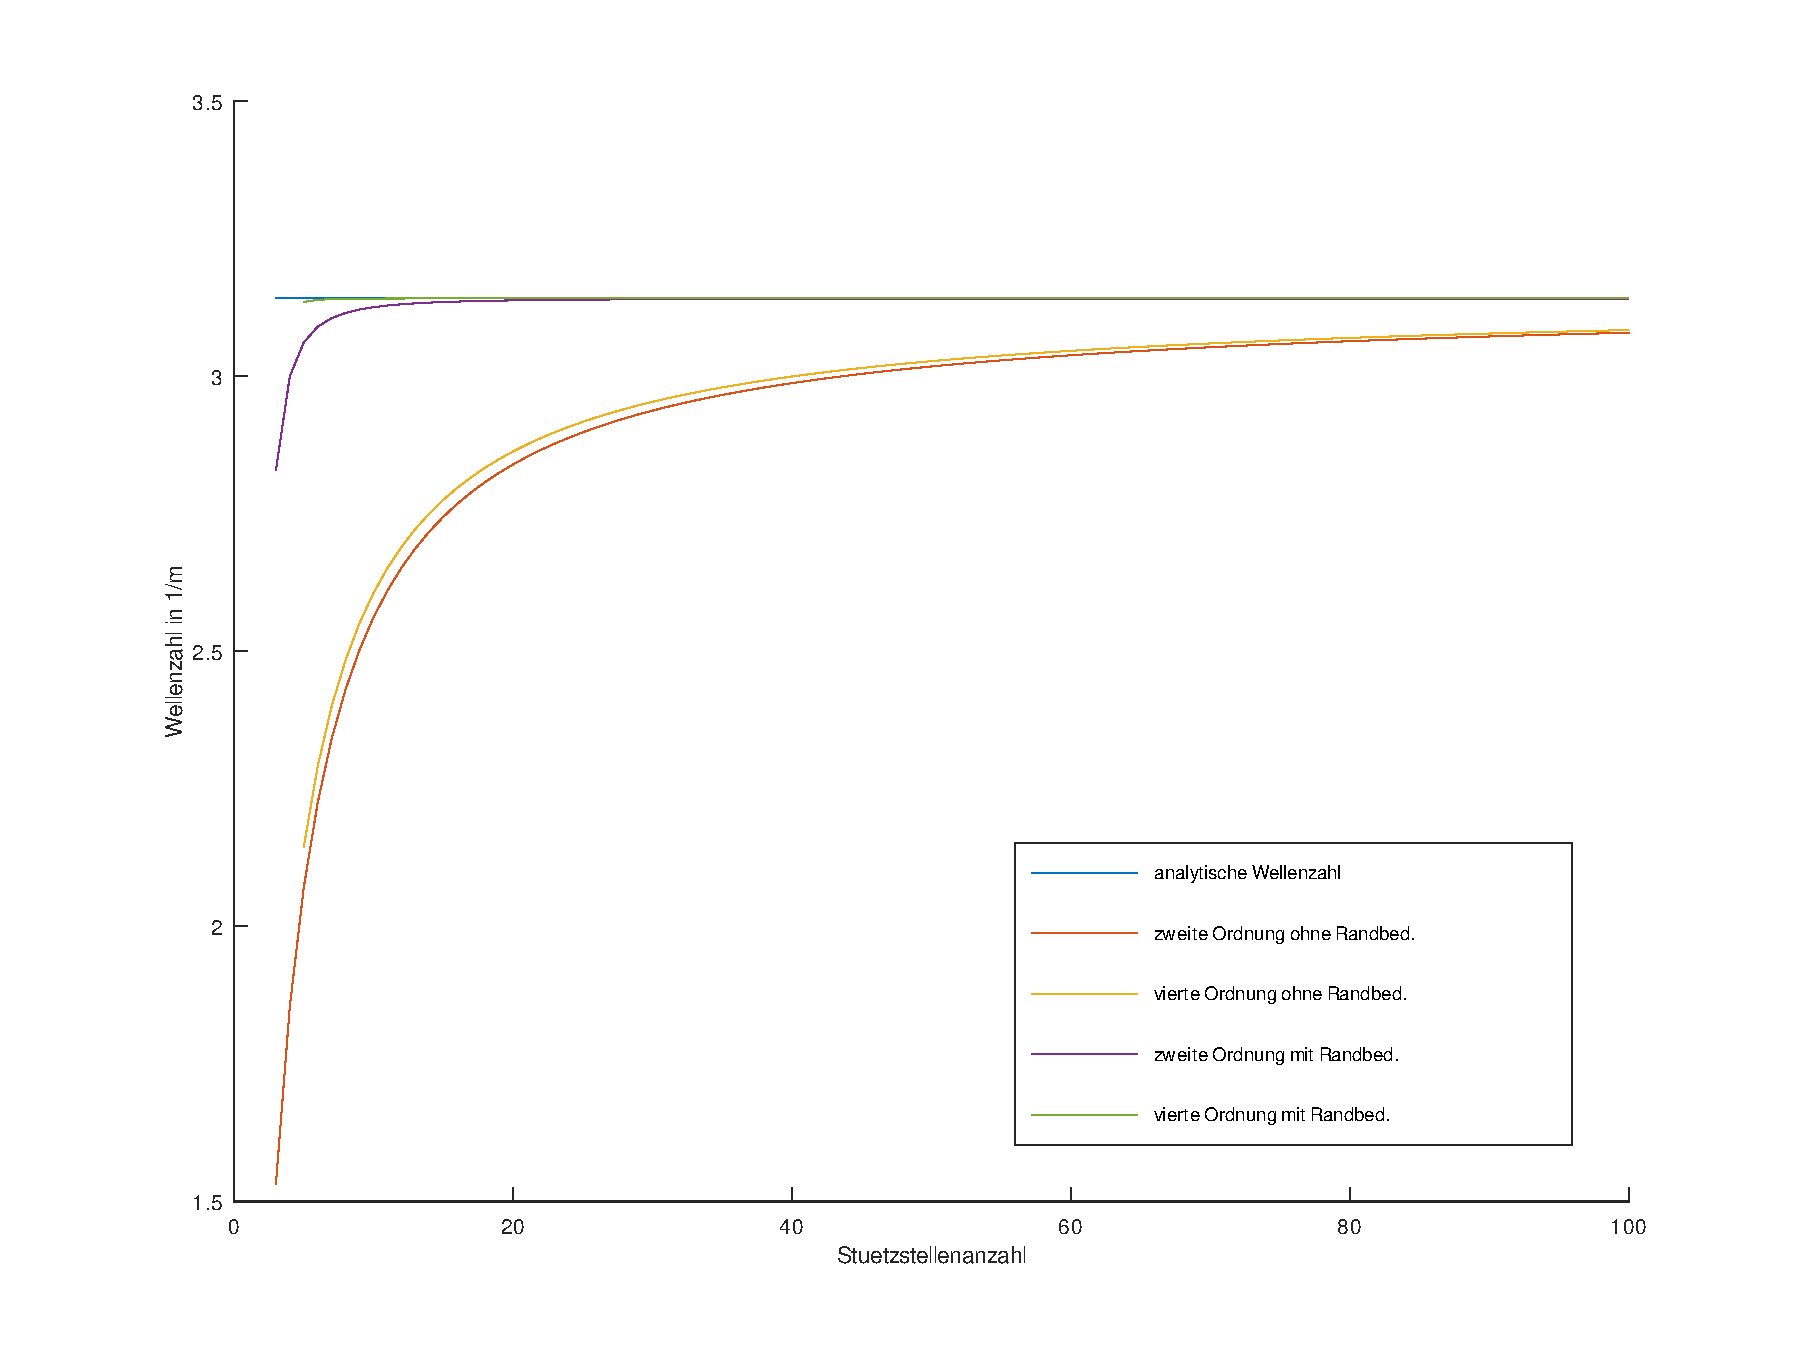
\includegraphics[trim = 25mm 10mm 25mm 15mm, clip, width=0.7\textwidth]{plotConv.pdf}
		\caption{Approximation der Wellenzahl in Abhängigkeit der Stützstellenanzahl des Gitters.}
		\label{Abb:plotCov}
	\end{figure}
	\noindent
	\begin{figure}[h]
		\centering
		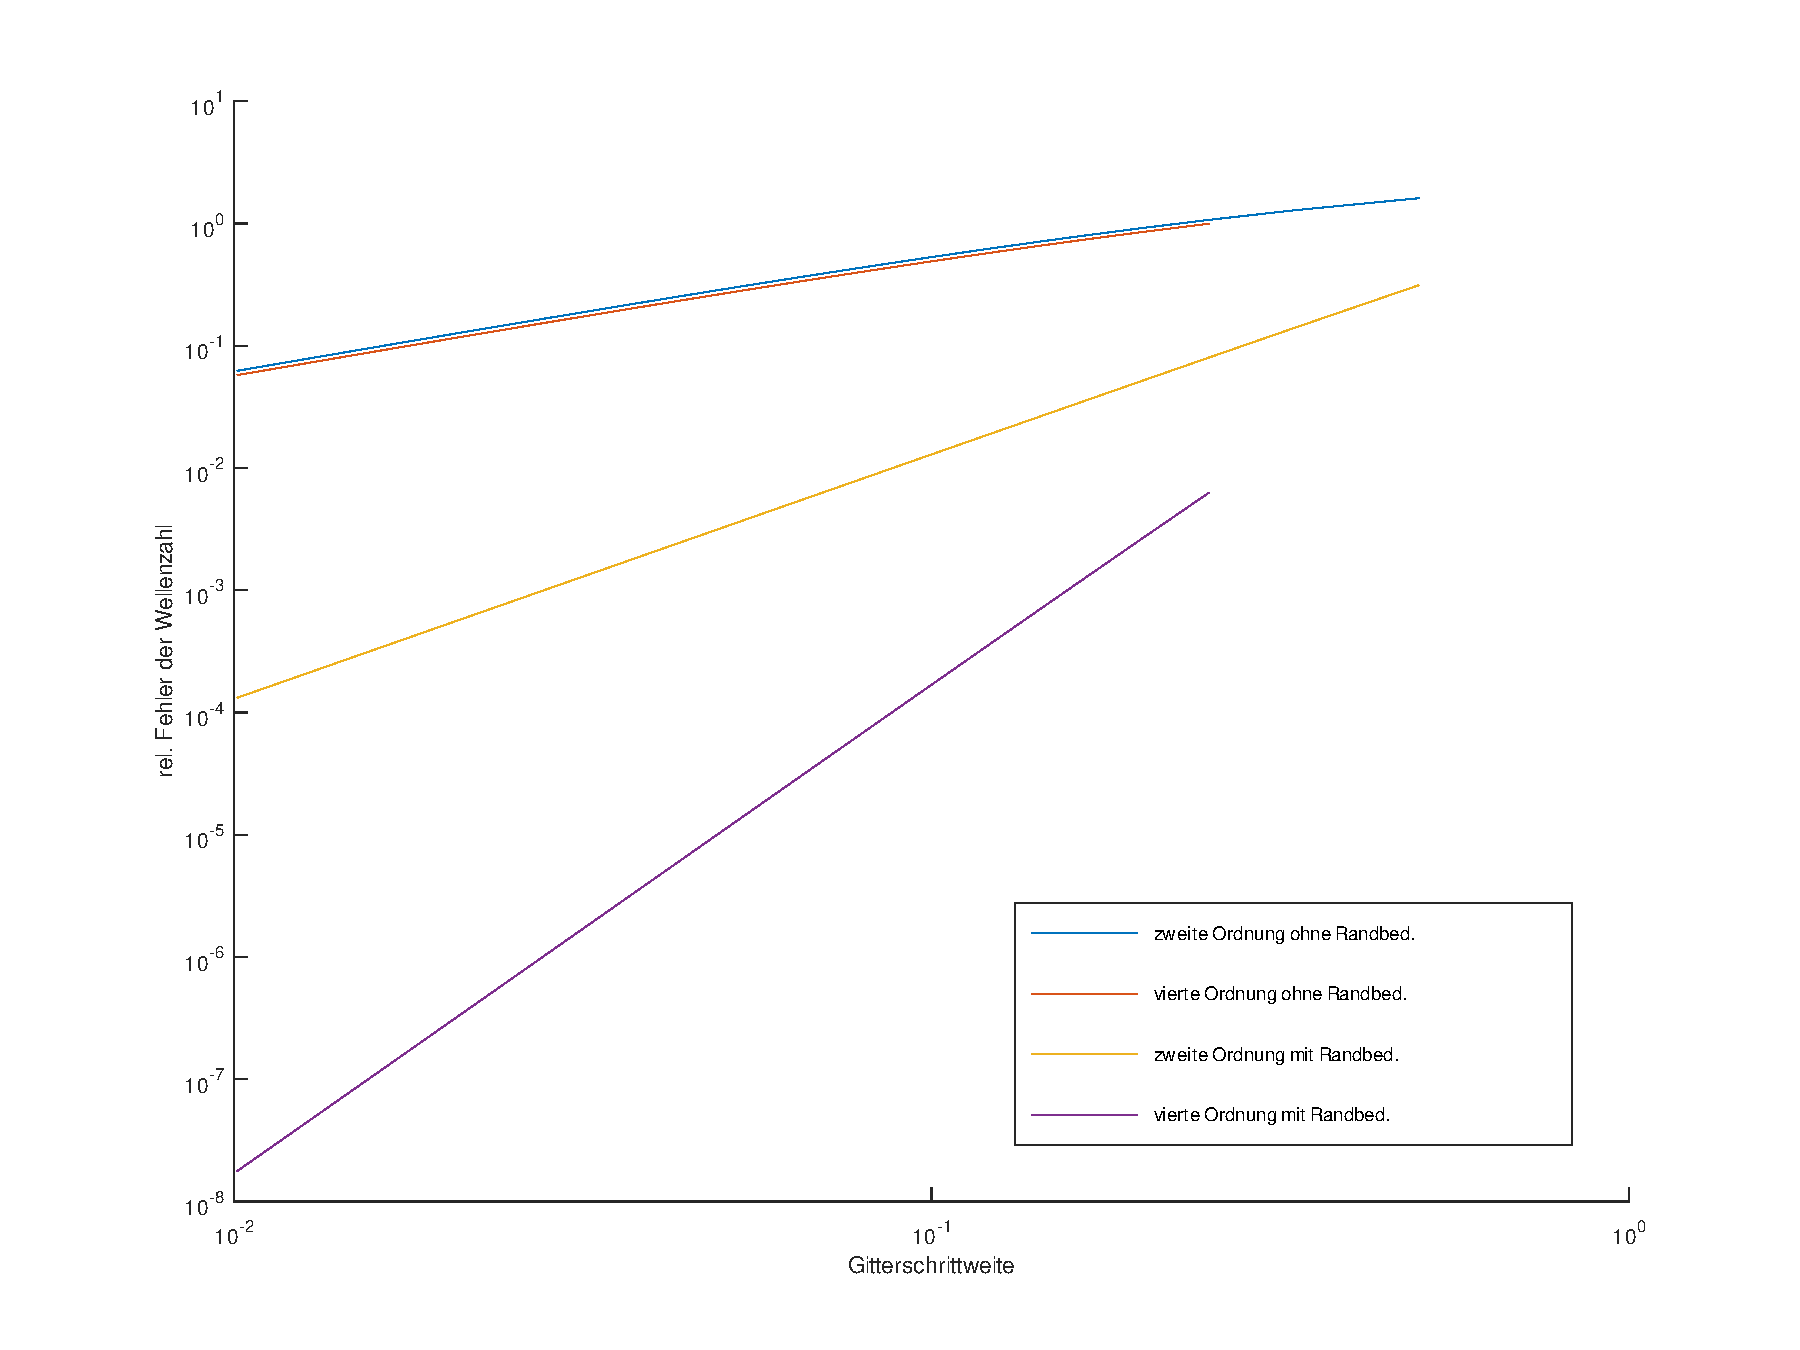
\includegraphics[trim = 25mm 10mm 25mm 15mm, clip, width=0.7\textwidth]{plotConvloglog.pdf}
		\caption{Wellenzahlfehler in Abhängigkeit der Gitterschrittweite.}
		\label{Abb:plotCovloglog}
	\end{figure}
	
	
	%\lstinputlisting {plotConv.m}
	

	{\subsection{Dreidimensionale Darstellung}}
	
	% --> Aufgabe
	\begin{framed}
		\noindent \textbf{6.} Schreiben Sie ein Skript \lstinline{plotCyl}, welches den Zylinder aus der Vorbereitung visualisiert.
		Bauen Sie hierzu auf der \matlab-Funktion \lstinline{patch} auf. Verwenden Sie die Anzahl der Dreiecksflächen
		in einer Deckelfläche \lstinline{nd=20}, den Radius \lstinline{r=1} und die Höhe \lstinline {h=1}.\label{exer:plotCyl}
	\end{framed}
	\noindent
	Zur Lösung dieser Aufgabe wurde der Pseudocode aus Aufgabe 7 umgesetzt und die dabei gewählten Verfahren implementiert. Der Zylinder ist in Abbildung \ref{Abb:plotCyl} zu sehen.
	\begin{figure}[h]
		\centering
		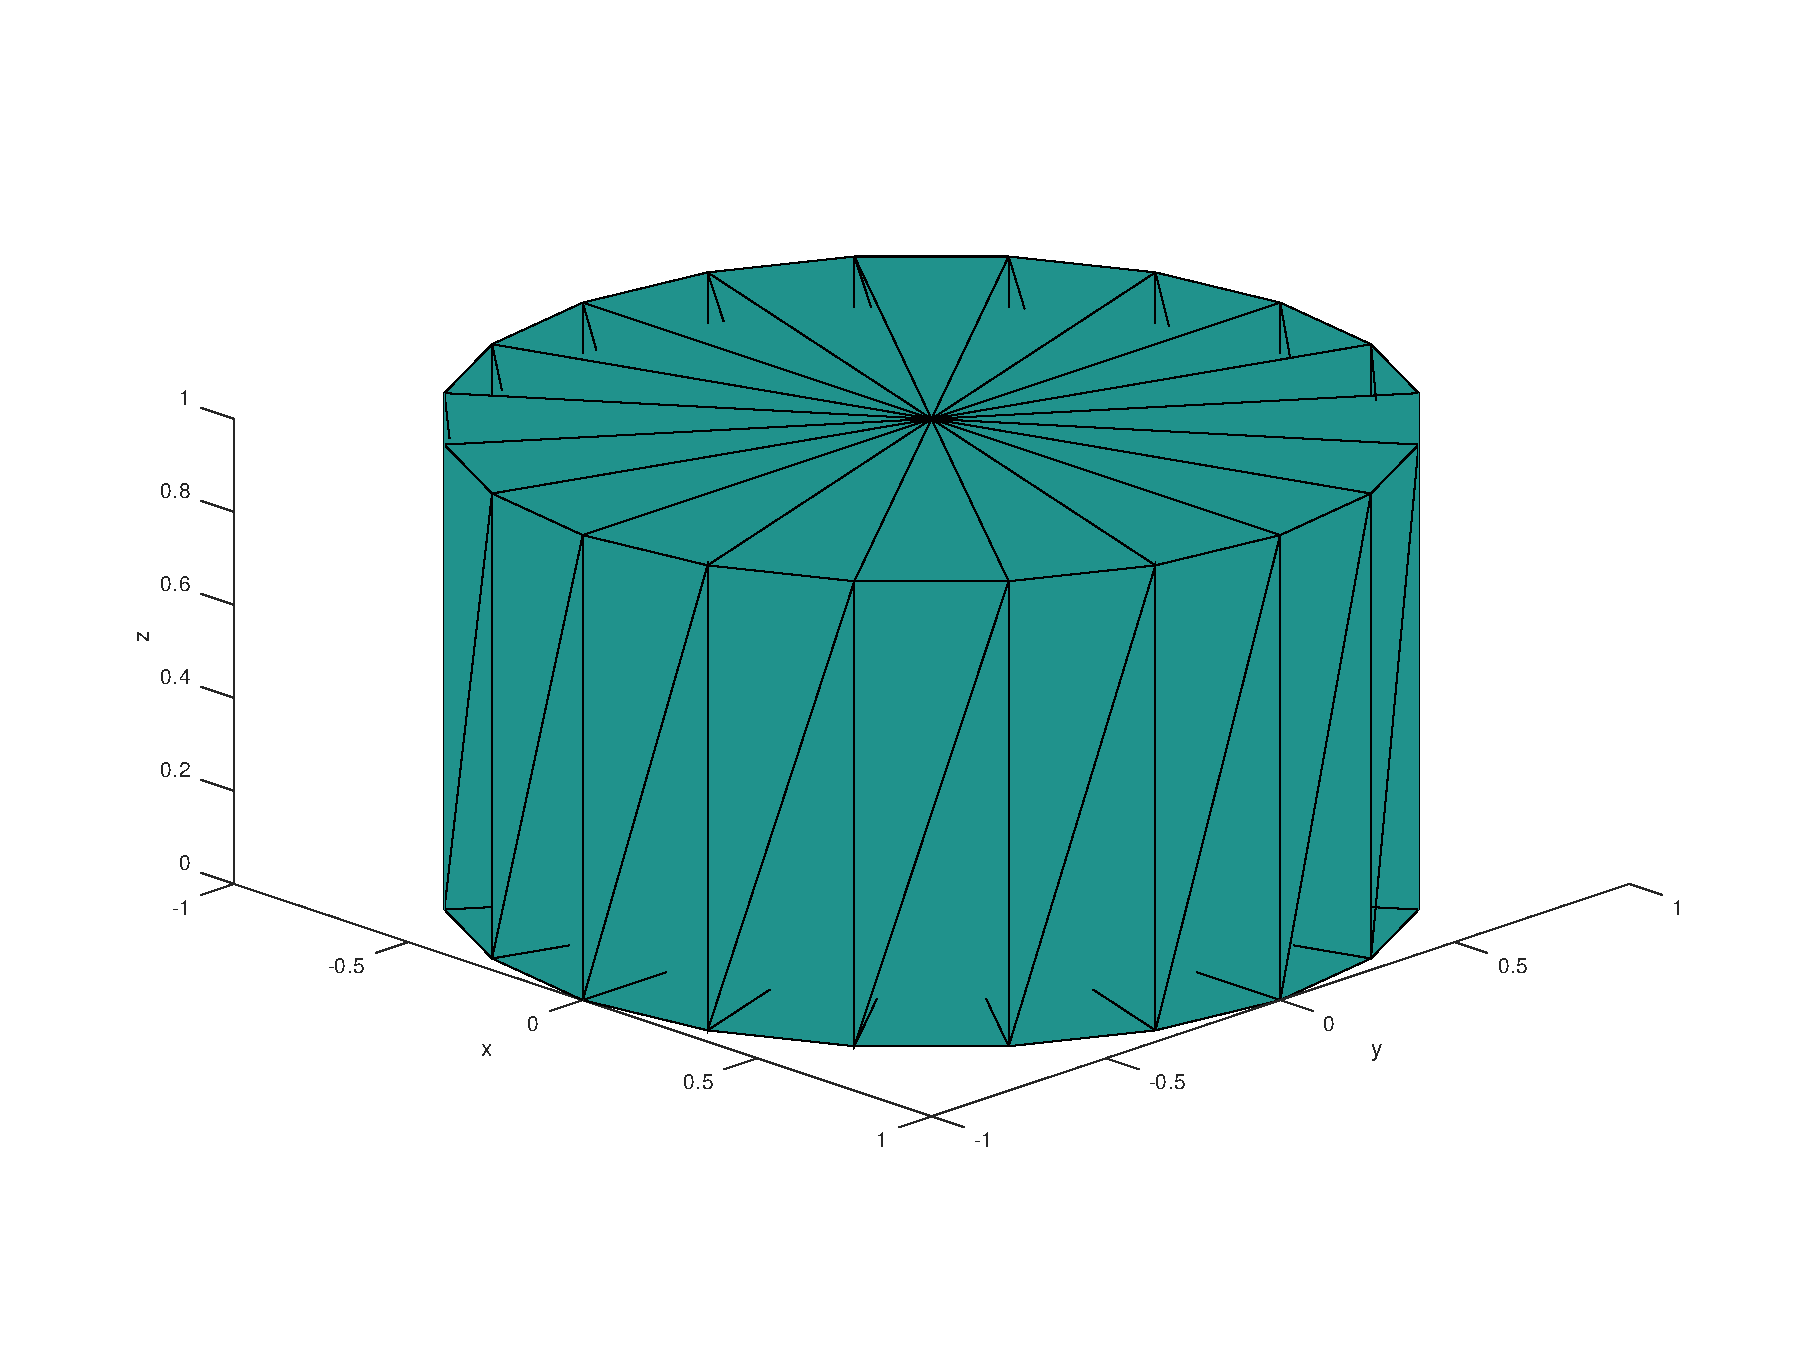
\includegraphics[trim = 25mm 10mm 25mm 25mm, clip, width=0.7\textwidth]{plotCyl.pdf}
		\caption{Nach den Vorgaben geplotteter Zylinder.}
		\label{Abb:plotCyl}
	\end{figure}
	
	%\lstinputlisting {plotCyl.m}
	
	% --> Aufgabe
	\begin{framed}
		\noindent \textbf{7.} Stellen Sie für einen Zylinder Ihrer Wahl den Oberflächenfehler $\Delta A$ sowie den Volumenfehler $\Delta V$ in Abhängigkeit von der Anzahl der Dreiecksflächen je Deckel $n_\text{D}$ (Vorbereitungsaufgabe \ref{exer:deltaAdeltaV}) in einem Skript
		\lstinline{plotVisErr} doppelt-logarithmisch dar.   Mit welcher Ordnung konvergieren die Fehler?
		Aus der Vorbereitung wissen Sie zusätzlich, wie der Speicherbedarf der
		Darstellung skaliert.\\
		Wie viele Dreiecke sind notwendig um einen Diskretisierungsfehler kleiner als $10^{-5}$ zu garantieren?\label{exer:plotVisErr}
	\end{framed}
	\noindent
	%\lstinputlisting {plotVisErr.m}
	In Abbildung \ref{Abb:plotVisErr} ist der relative Oberflächen- und Volumenfehler in Abhängigkeit der Dreiecke auf der Deckelfläche dargestellt. Um ein Fehler kleiner von $10^{-5}$ zu garantieren, benötigt man 812 Dreiecke.
	\begin{figure}[h]
		\centering
		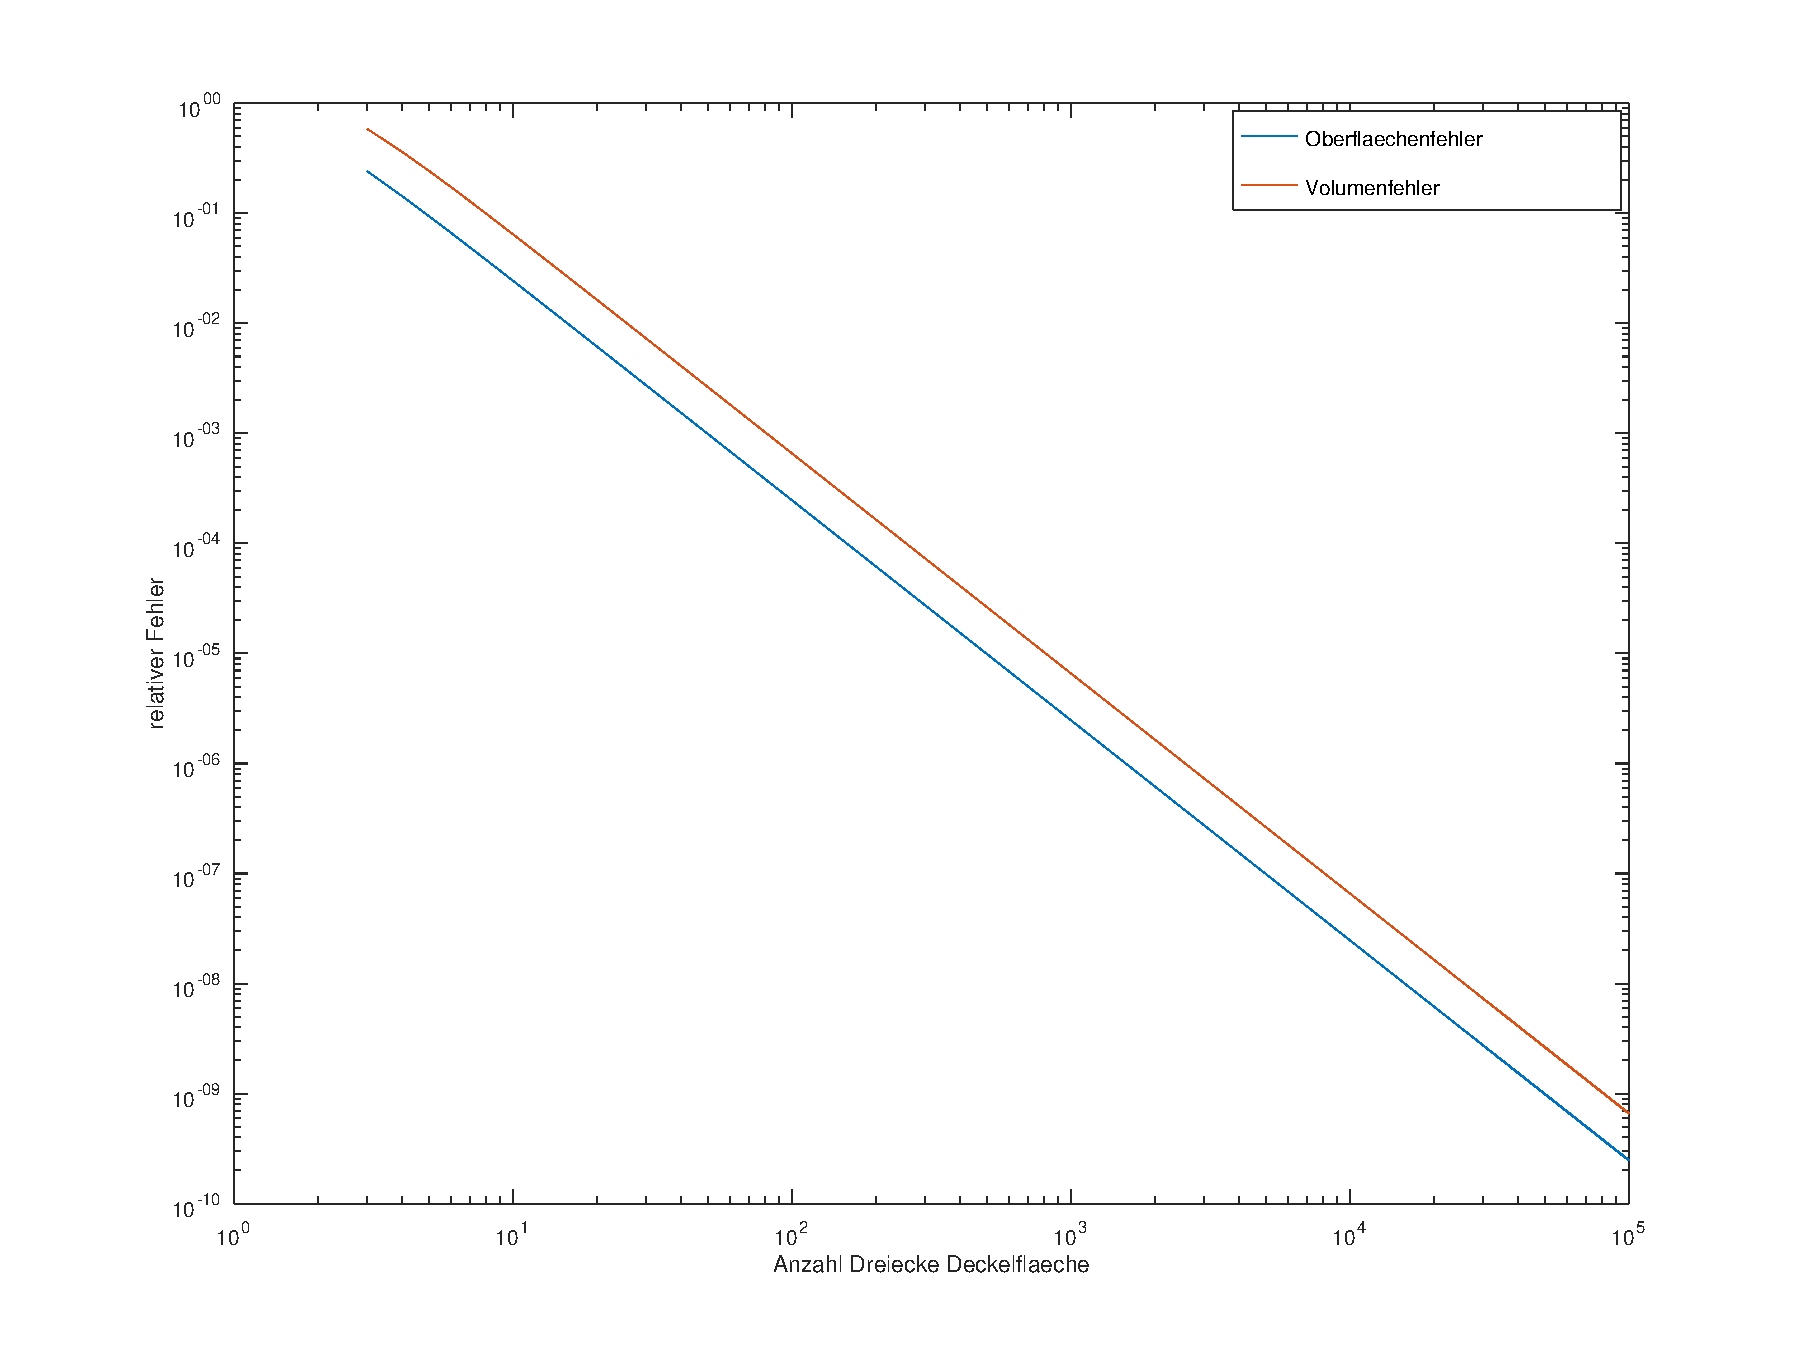
\includegraphics[trim = 25mm 10mm 25mm 15mm, clip, width=0.7\textwidth]{plotVisErrloglog.pdf}
		\caption{Relativer Oberflächen- und Volumenfehler in Abhängigkeit der Dreiecke auf der Deckelfläche.}
		\label{Abb:plotVisErr}
	\end{figure}
	
	% --> Aufgabe
	\begin{framed}
		\noindent \textbf{8.} Verwenden Sie die bereitgestellte Methode \lstinline{read_stl} um zwei der bereitgestellten Geometrien im STL-Format (vgl.~Abb.~1.4) einzulesen und dann erneut mit \lstinline{patch} darzustellen.
		Nennen Sie Ihr Skript \lstinline{plotStl}.\label{exer:plotStl}
	\end{framed}
	
	%\lstinputlisting {plotStl.m}
	
	%-------------------- Ende der Aufgaben --------------------
	
	\section{Fazit}
	Wie man in den Aufgaben sehen konnte, kann man durch die Bildung von Matrizen (Diskretisierungen) für die Ableitungsoperatoren die gegebenen Gleichungen einfach numerisch lösen. Auch bei der Diskretisierung von Oberklächen wurde erkannt, dass Matrizen hier ein einfach zu handhabendes Speichermedium bilden. Die Diskretisierung kann man schnell, aber auch relativ genau bestimmen.
	
\end{document}
